\chapter{Methods}
\%3CmxGraphModel%3E%3Croot%3E%3CmxCell%20id%3D%220%22%2F%3E%3CmxCell%20id%3D%221%22%20parent%3D%220%22%2F%3E%3CmxCell%20id%3D%222%22%20value%3D%22%26lt%3Bfont%20color%3D%26quot%3B%23ffffff%26quot%3B%26gt%3B%26lt%3Bb%26gt%3Btrain%26lt%3Bbr%26gt%3B%26lt%3B%2Fb%26gt%3B%26lt%3B%2Ffont%26gt%3B%22%20style%3D%22shape%3Dnote%3BwhiteSpace%3Dwrap%3Bhtml%3D1%3BbackgroundOutline%3D1%3BdarkOpacity%3D0.05%3BfillColor%3D%234D4D4D%3B%22%20vertex%3D%221%22%20parent%3D%221%22%3E%3CmxGeometry%20x%3D%22340%22%20y%3D%22315%22%20width%3D%2280%22%20height%3D%22100%22%20as%3D%22geometry%22%2F%3E%3C%2FmxCell%3E%3C%2Froot%3E%3C%2FmxGraphModel%3Elabel{chapter:methods}
\section{Dataset}
The dataset was created by Dr. Tichy and his team using the Computer Vision Annotation Tool (CVAT). It has been extended and improved multiple times over the course of this work, and there is still ongoing work. At the time of writing this report, it consisted of 2599 bitewing X-ray images with 4575 annotations of tooth decay. Out of those, there are 890 images without any decay. The distribution of dental caries per image is depicted in the figure \ref{fig:hist_caries_per_img}. For clarity reasons, we omitted six images that contained more than ten caries. From the histogram on the figure \ref{fig:hist_caries_dim}, we observe that most caries have dimensions between 10 and 75 pixels. However, there are outliers as big as 380 pixels per dimension. This diversity is increasing the difficulty of the task.

We used the COCO data-format to store data, and adapted this format even in the implementation only with rare exceptions when custom data-format was needed. During the experiments, we used the 70:15:15 split into training, validation and test dataset.
\begin{figure}
    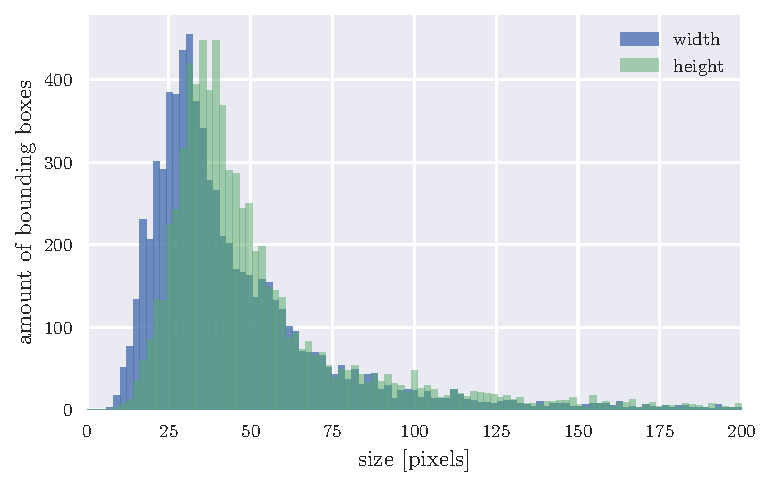
\includegraphics[width = \linewidth]{images/dataset_histogram.pdf}
    \caption{Histogram of bonding boxes dimensions in the dataset}
    \label{fig:hist_caries_dim}
\end{figure}

\begin{figure}
    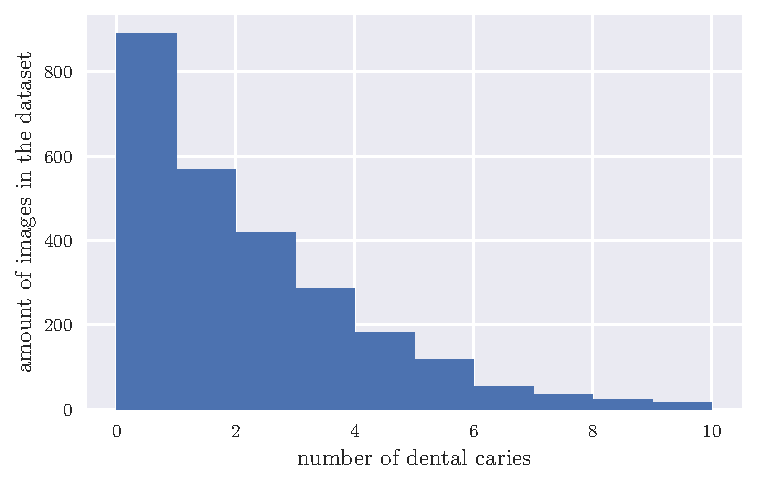
\includegraphics[width=\linewidth]{images/caries_histogram.pdf}
    \caption{Histogram of the amount of dental caries per image}
    \label{fig:hist_caries_per_img}
\end{figure}
\subsubsection{Image augmentations}
The image was augmented by a single pipeline that applied the following transformations with corresponding probabilities p.
\begin{itemize}
    \item Normalize by substracting the mean of the dataset and dividing by standard deviation of the dataset, $p=1$
    \item Resize and pad to $1024\times1024$, $p=1$
    \item Horizontal flip, $p=0.5$
    \item Vertical flip, $p=0.5$
    \item Rotation, $p=0.3$, rotation limit$=10^{\circ}$
    \item Translation, $p=0.5$, translation limit$=10\%$ of the image size
    \item Gaussian blur flip, $p=0.3$, kernel size from 7 to 31
    \item Gamma correction, $p=0.3$, $\gamma$ in range from 0.6 to 1.4
\end{itemize}

The result of those augmentations can be seen in the appendix \ref{appendix:img_transformations}.
\subsubsection{Computing power}
All the computations were realized on the CMP cluster, consisting of multiple GPU nodes. The experiments were conducted on the Boruvka and Zorn machines. Both of them have 32 CPU cores, 256GB of RAM memory, and 8 NVIDIA GeForce GTX 1080-Ti graphics cards with 12GB of dedicated memory.

\subsection{Neural network models}
\subsubsection{YOLOv5}
The YOLOv5 architecture was used with the 5l6 backbone. That is the second-largest backbone from the sixth generation of the backbone architectures. When experimenting with YOLOv5 we used a batch size of 3, which was the maximal size, that could fit into the GPU memory.
\subsubsection{EfficientDet}
We used the EfficientDet-D4 because it was proposed as the optimal-efficiency architecture to use for image size of 1024 pixels \cite{Tan2019}. Even though there are three bigger backbones available, the batch size has to be 1 for the network to fit into the GPU. This removed the option of trying more parameter-heavy backbones.

\subsubsection{Optimizers}
The Adam optimizer was used during all experiments. The parameters $\beta_1, \beta_2$ were set to 0.9 and 0.999 and weight decay was chosen to be $1e^{-6}$. Since we could not fit a reasonably big batch size into the GPU, the optimization step was performed every four forward passes. This should emulate a bigger batch size and increase the chance of finding global optimization minima.
\subsubsection{Learning rate}
The initial value of the learning rate was set to $1e^{-5}$ and reduced on plateau learning rate scheduler was used. The monitored value by the scheduler was validation loss, and the learning rate decreased by the factor of 5 when the improvement of the loss stalled for five consecutive epochs.
\subsubsection{Termination condition}
The training was halted when the validation error did not decrease over the course of 10 epochs, but not earlier than after 50 epochs from the beginning of the training.


\section{Dental-restorations segmentation segmentation}
\subsection{Non-deeplearning approach}
We decided to test the approach, that was proposed by Abdalla-Aslan and Yeshua \cite{AbdallaAslan2020,Yeshua2019} as described in section \ref{sec:related_works:dental_restorations}. This means, that we defined a pipeline of image processing operations, where we:
\begin{itemize}
    \item Threshold the image: We tried Otsu's thresholding method, Gaussian and mean adaptive thresholding methods where we tested different kernel sizes $K_t$ and threshold values $T$.
    \item Removed predicted pixels at the border of X-ray image: Bitewing X-ray images usually do net have a ractangular shape as can be seen in \ref{fig:bitewing_sample}. This is a cause for hight contrast at the border of radigraph, which gets detected by adaptive thresholding methods. We therefore detect the image pading and morphologically dilate it by square kernel of size $K_b \times K_b$. Border pixels obtained by dilation are remoed from the thresholded image.
    \item Morphological openning: To filter out falsely detected regions we apply morphological openning, for this purpose we use square-shaped kernel with size $K_o$.
\end{itemize}

The pipeline deffined above has four hyper-parameters to be tuned. We therefore define a grid-shaped search space as can be seen in table \ref{tab:hyper_param_segmentation}. The dataset was split into two equaly-sized parts, called tune and test. For each set of hyer-parameters we evalueted the IOU metric on each image of the tune part of the dataset. We selected best hyper-parametrs based on the average IOU value and used those to evaluate on the test-part of the dataset.

as can be seen in table \ref{tab:hyper_param_segmentation}
\begin{table}
    \begin{tabular}{|c|c|c|c|}
        \hline
        Hyper-parameter & minimal value & maximal value & step \\ \hline
        $K_t$           & 3             & 153           & 10   \\ \hline
        $T$             & 1             & 11            & 2    \\ \hline
        $K_b$           & 41            & 101           & 20   \\ \hline
        $K_o$           & 1             & 51            & 5    \\ \hline
    \end{tabular}
    \caption{Hyper-parameter search space for restorations segmentation pipeline}
    \label{tab:hyper_param_segmentation}
\end{table}

\subsection{Deep-learning approach}
The dataset was splited in training, validation and test part with 70:15:15 ratio. For the training part of the dataset we used image augmentations described in TODO. For the validation and test part of the dataset we only normalized the image by TODO.
We used default U-Net architecture model with depth 5. As a loss function we used binary cross-entropy. Learning rate with value of 1e-2 was used and reduce on plateu scheduler was used. The model was trained for 50 epochs and at the end we selected the best model according to IOU on the validation dataset.

We used post-processing methods on the best-performing model.



\section{Model ensembling}

For every model in the table TODO we loaded weights used to obtain the results in the table and generated predictions on train, test and validation part of the dataset. When predicting, each image was rescaled to size required by corresponding model and normalized. This lead to predictions beeing in the space of the transformed image. Therefore we used inverse transformation to the rescaling, to obtain coordinates in the original image. This allows us to combine predictions regardless the model architecture.
Predictions were saved into file named predictions\_\{model architecture\}\_\{model backbone\}.json.

Confidence values maximizing F1 score differ across models $m$, we therefore normalize them by the following formula:
\begin{align}
    s_{j,i} = \frac{s_{j,i} \max_l S_l}{  S_j}, \quad j \in \{ 1,...,m\}, i \in {1,...,n_j}
\end{align}

We perform ensembling by the approach described in section TODO. We firstly tryed to estimate weights for ensembling from resutls of individual models and as threshold value $T$ and $sigma$ selected values proposed by authors of the ensembling method.

We performed grid search over hyper-paramers in to following manner: Defined parameter search space, which can be seen in talbe \ref{tab:ensembling_search_space}. We evaluated $AP@.5$ on every image of the validation datasaet and averaged those values. The best hyper-parameters were selected and we used them for evaluation on test dataset. The whole worflow is shown in figure \ref{fig:diag:ense_search}.

\begin{table}
    \centering
    \begin{tabular}{|c|c|c|c|}
        Parameter                                         & minimal value & maximal value & step \\ \hline
        Model weight                                      & x             & x             & x    \\ \hline
        IOU $T$                                           & x             & x             & x    \\ \hline
        Sigma & x             & x             & x    \\ \hline
    \end{tabular}
    \caption{Hyper parameter search-space for model ensembling}
    \label{tab:ensembling_search_space}
\end{table}

We changed the equation TODO to:
\begin{align}
    a = foo
\end{align}
We performed the grid-search again, but the number of parameters grew significantly, so that grid-search became commputationaly untractable. We therefore used optuna optimization library to perform this task. The search space is in table \ref{tab:ensembling_search_space_area}, please note, that the search space became continuous in contrast to the previous.

\begin{table}
    \centering
    \begin{tabular}{|c|c|c|}
        Parameter                                         & minimal value & maximal value \\ \hline
        Model weight (small, medium, large)               & 0.01          & 1             \\ \hline
        IOU $T$                                           & 0.05          & 1             \\ \hline
        Sigma\footnote{Soft non-maximal superssion only } & x             & x             \\ \hline
    \end{tabular}
    \caption{Hyper parameter search-space for model ensembling}
    \label{tab:ensembling_search_space_area}
\end{table}

We used results from table TODO and normalized all confidence values o
\begin{figure}
    \centering
    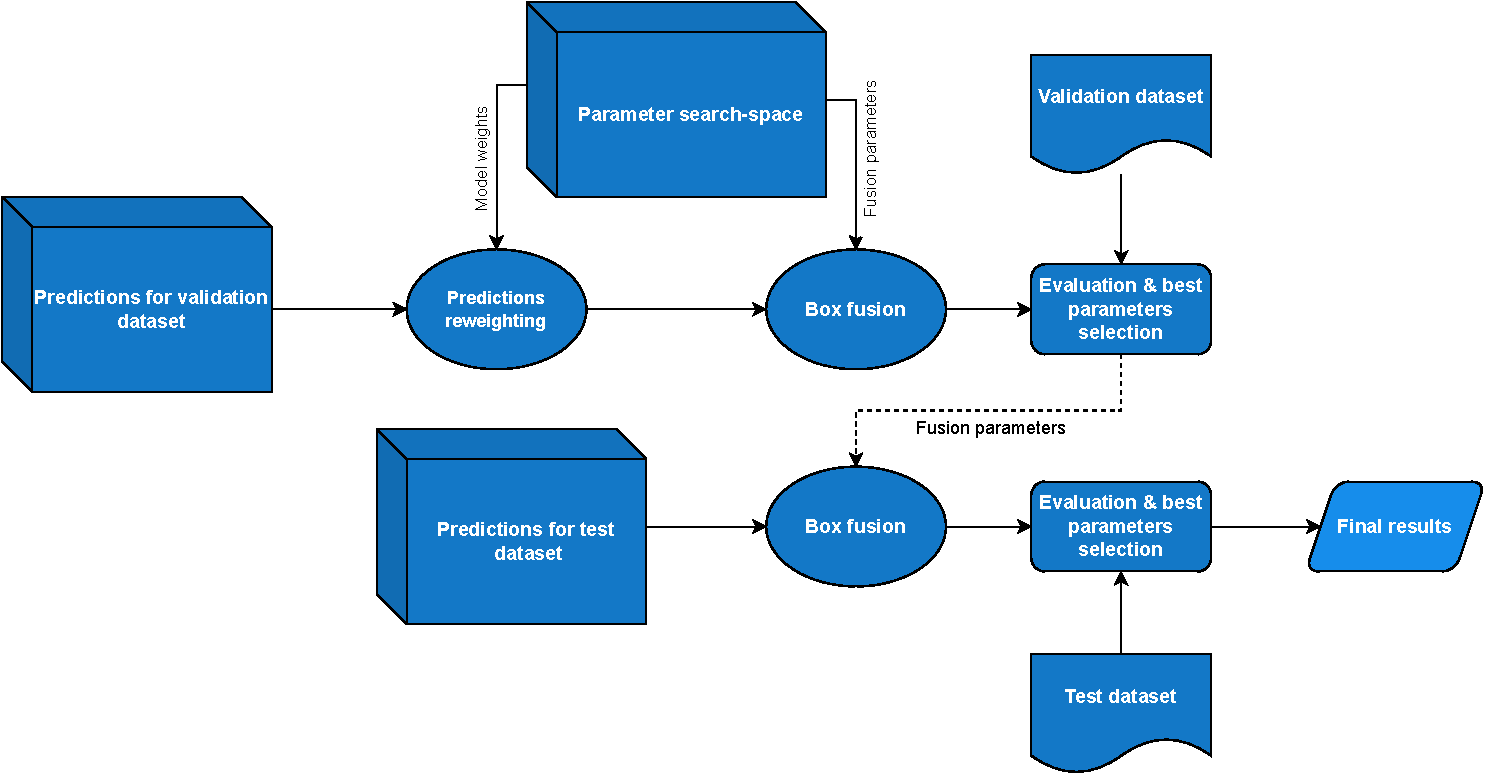
\includegraphics[width=\linewidth]{images/ensemble_search_diag.drawio.pdf}
    \caption{Schematics of the search of hyper-parametrs and weights for ensembling}
    \label{fig:diag:ense_search}
\end{figure}

\begin{figure}
    \centering
    \begin{lstlisting}[language=json, numbers=none]
   {"filename" : {
       "bboxes" : [[x1, y1, x2, y2],...],
       "labels": [l1, l2,...],
       "scores": [s1, s2,...],
       "stage" : "test" / "val" / "train"
       },
    "filename2" : {...},
    ...
   }
\end{lstlisting}
    \caption{Structure of the data in .json file used to store model predictions}
    \label{fig:predictions_json}
\end{figure}